In this section, we will analyze how several
model parameters affect the system's performance.
First, we will examine the effect of the number of bleedings.
Next, we will analyse the effect of the number of reheatings.
Finally, the effect of the pressure at the high-pressure turbine inlet
will be discussed.

\subsection{Influence of the number of bleedings}

To analyse the influence of the number of bleedings, we varied
the number of bleedings in the low-pressure turbine from $0$ to $5$.
With the number of bleedings in the intermediate-pressure and high-pressure turbines kept constant,
this adjustment allowed the total number of bleedings to range from $5$ to $10$.
Our results are presented in figure \ref{fig:bleedings_results}.

\begin{figure}[H]
    \centering
    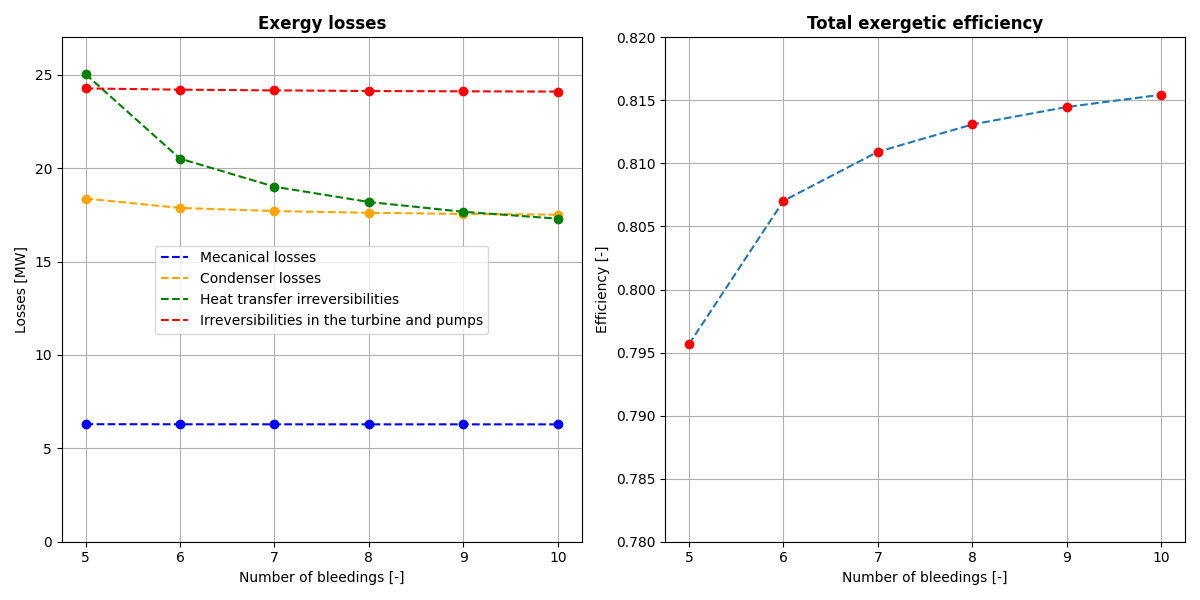
\includegraphics[width=0.5\textwidth]{Figures/bleedings.png}
    \caption{Influence of the number of bleedings on the system's performance.}
    \label{fig:bleedings_results}
\end{figure}

\noindent \textbf{Analysis :} As expected, the total exergetic efficiency 
increases with the number of bleedings but this increase is not linear and 
tends to saturate.  At one point, the costs related to the installation of 
an additional bleeding will exceed the benefits in terms of efficiency.
This benefit can be explained by three main factors :
\begin{enumerate}[noitemsep]
    \item When a bleeding is extracted from the turbine, the mass flow rate of steam 
    entering the condenser is reduced.  This reduces the exergy losses at the condenser ($p_{condex}$).
    \item The losses due to irreversibilities in the heat exchangers ($p_{transex}$) 
    are reduced because the extracted steam preheats the feedwater in stages, 
    lowering the temperature difference and minimizing exergy destruction.
    \item The mechanical losses ($p_{mec}$) and the losses due to irreversibilities in 
    the turbine and pumps ($p_{rotex}$) remain more or less constant.
\end{enumerate}
Consequently, as the number of bleedings increases, the overall exergy destruction in the cycle is reduced.\\


\noindent \textbf{Remark :} For this analysis, the total exergetic efficiency ($\eta_{totex}$)
is defined as follows ;
$$\eta_{totex} = \frac{P_e}{P_e + p_{transex} + p_{rotex} + p_{condex} + p_{mec}}$$
we obtain relatively high values ($\approx 80\%$) because the chimney losses, combustion
irreversibilities and heat transfer irreversibilities in the 
steam generator are not considered.

